\documentclass[a4paper,french]{paper}
\usepackage{../../_latex_assets/villemejane_iogs_ceti}

%Informations about this document 
%------------------------------------------
\def\module{Conception Electronique pour le Traitement de l'Information}
\def\moduleAbrege{5N-027-SCI / CéTI}
\def\annee{}

\def\titre{Bloc 1 / Capteurs et mise en forme / CORRECTION}
\author{Julien VILLEMEJANE}

\subtitle{Bloc 1}
\institution{LEnsE / Institut d'Optique Graduate School}

\title{\titre}
\usepackage{circuitikz} 

\begin{document} 
%Beginning First Page. 
%------------------------------------------
\enteteThematiqueObligatoire{}

%Beginning Content. 
%------------------------------------------

%%%%%%%%%%%%%%%%%%%
\encadreTDExo{1.1 - Abaisser une tension}{
Proposer un circuit permettant d'abaisser une tension d'un facteur $k$.

$0 < k < 1$ 
}

Pour réduire une tension, il est possible d'utiliser un \textbf{pont diviseur de tension}, basé sur l'utilisation de 2 résistances en série comme proposé dans le schéma suivant.

\medskip

\begin{center}
\begin{circuitikz}
	\draw (1,0) to [short, *-] (3,0)
		to[R=$R_{2}$, -*] (3,2)
		to[R=$R_{1}$, -] (3,4)
		to [short, -*, i<_=$I$] (0,4);
	\draw (3,0) to[short, -o] (4,0);
	\draw (3,2) to[short, -o, i=$I_S$] (4,2);
	
	% fleche
	\draw (0,0.5) edge[->] (0,3.5);
	\node (Ein) at (-1,2.25){$V_E$};

	\draw (0,0) to [short, *-] (1,0)
		node[ground](GND){};
	% fleche
	\draw (3.5,0.3) edge[->, green!40!black] (3.5,1.7); \node[text=green!40!black] (US) at (4,1){$V_S$};
\end{circuitikz}
\end{center}

Pour le calcul, on peut s'intéresser au courant $I$ en écrivant deux lois des mailles différentes :

\begin{enumerate}
	\item $V_E - R_1 \cdot I - R_2 \cdot I = 0$
	\item $V_S - R_2 \cdot I = 0$
\end{enumerate}

Cela suppose que l'on considère que le courant $I_S = 0$.

En combinant les deux, on obtient la relation entre $V_E$ et $V_S$ suivante : $$V_S = V_E \cdot \frac{R_2}{R_1 + R_2}$$

\noindent\hrulefill

\newpage

Si on suppose maintenant que le circuit précédent est chargé par une résistance $R_L$, on obtient alors le montage suivant :

\begin{center}
\begin{circuitikz}
	\draw (1,0) to [short, *-] (3,0)
		to[R=$R_{2}$, -*, i<_=$I_2$] (3,2)
		to[R=$R_{1}$, -] (3,4)
		to [short, -*, i<_=$I$] (0,4);
	\draw (3,0) to[short, -o] (4,0);
	\draw[dashed] (4,0) to[short, -] (5.5,0) 
		to[R=$R_L$, -] (5.5,2)
		to[short, -] (4,2);
	\draw (3,2) to[short, -o, i=$I_S$] (4,2);
	
	% fleche
	\draw (0,0.5) edge[->] (0,3.5);
	\node (Ein) at (-1,2.25){$V_E$};

	\draw (0,0) to [short, *-] (1,0)
		node[ground](GND){};
	% fleche
	\draw (3.5,0.3) edge[->, green!40!black] (3.5,1.7); \node[text=green!40!black] (US) at (4,1){$V_S$};
\end{circuitikz}
\end{center}

Dans ce cas, le courant $I_S$ n'est plus nul.

Le courant $I$ traversant $R_1$ va alors se partager entre $R_2$ et $R_L$. On aura alors la seconde loi des mailles écrites précédemment qui ne sera plus valide.

On peut alors écrire les relations suivantes :
\begin{enumerate}
	\item loi des mailles : $V_E - R_1 \cdot I + V_S$ 
	\item loi des mailles : $V_S - R_L \cdot I_S = 0$  
	\item loi des noeuds : $I = I_S + I_2$ 
	\item loi des mailles : $V_S - R_2 \cdot I_2 = 0$
\end{enumerate}

Après regroupement et simplification, on obtient la relation suivante : $$V_S = V_E \cdot \frac{R_{eq}}{R_1 + R_{eq}}$$  

avec $R_{eq} = \frac{R_2 \cdot R_L}{R_2 + R_L}$ (mise en parallèle de $R_2$ et $R_L$).
 

\newpage
%%%%%%%%%%%%%%%%%%%
\encadreTDExo{1.2 - Élever une tension}{
Proposer un circuit permettant d'élever une tension d'un facteur $k$.

$k > 1$
}

Pour pouvoir élever une tension, il est nécessaire d'\textbf{apporter de l'énergie au montage}. Une solution possible est l'utilisation d'un amplificateur opérationnel (ou amplificateur linéaire intégré - ALI).

On peut par exemple utiliser un montage de type amplificateur non-inverseur dont le schéma est fourni ci-dessous :

\begin{center}
\begin{circuitikz}
	\draw (0,0) node[above]{} to[short, o-, i=$i^+$] ++(1,0)
	node[op amp, noinv input up, anchor=+, fill=blue!10!white](OA){\texttt{AOP1}}
	(OA.-) to[short,-, i<_=$i^-$] ++(0,-1) coordinate(FB)
	to[R=$R_1$, i=$I_1$] ++(0,-2.3) node[ground]{}
	(FB) to[R=$R_2$, *-] (FB -| OA.out) to[short,-, i<_=$I_2$] (OA.out)
	to [short, *-o] ++(1,0) node[above]{};
	\draw (0,-0.3) edge[<-,color={green!40!black}] (0, -4);
	\draw (0,-4.3) to[open,-o] ++(0,0) node[ground](GND){};
	\node[text={green!40!black}] (Ve) at (-0.5,-2.1){$V_E$}; 
	\draw (4.3,-1) edge[<-,color={red}] (4.3, -4);
	\draw (4.3,-4.3) to[open,-o] ++(0,0) node[ground](GND){};
	\node[text={red}] (Vs) at (4.8,-2.7){$V_S$}; 
\end{circuitikz}
\end{center}

Pour pouvoir faire le calcul de la fonction de transfert entre $V_S$ et $V_E$, il est nécessaire de faire \textbf{quelques hypothèses}.

La \textbf{première} vient du fait que les impédances d'entrée de tel amplificateur sont relativement grandes par rapport aux impédances des composants extérieurs ($R_1$ et $R_2$ ici). Les courants d'entrée $i^+$ et $i^-$ peuvent alors être négligés et considérés nuls.

La \textbf{seconde} hypothèse vient ici du fait que l'amplificateur a sa sortie rebouclé avec l'entrée inverseuse (-) par l'intermédiaire d'une résistance. Dans ce cas, on considère que le montage est en \textbf{fonctionnement dit linéaire}. Ainsi, on peut montrer que la différence de potentiel entre $V^+$ et $V^-$ tend vers 0. On peut alors considérer dans ce régime de fonctionnement, que $V^+ = V^-$.

\medskip

Il est alors possible par les lois habituelles de calculer le lien entre $V_S$ et $V_E$.

D'après la première hypothèse, on obtient que $I_1 = I_2$.

D'après la seconde hypothèse, on obtient que $V^- = V_E$.

En calculant le courant $I_1$ par la loi d'Ohm aux bornes de $R_1$, on obtient : $I_1 = \frac{V_E}{R_1}$.

De la même manière, on obtient : $I_2 = \frac{V_S - V_E}{R_2}$.

Après simplification, on obtient alors la fonction de transfert suivante : $$V_S = V_E \cdot \frac{R_1 + R_2}{R_1}$$


\noindent\hrulefill

\textbf{Attention !} Cette loi n'est cependant vraie qu'en basse fréquence et pour des tensions d'entrée faibles.

En effet, les amplificateurs linéaires intégrés sont des composants qui peuvent se modéliser comme un système de type \textbf{passe-bas}.

De plus, ils nécessitent d'être alimentés et lorsque la tension de sortie tend à dépasser la tension d'alimentation, on peut observer un \textbf{phénomène de saturation}.


\newpage
%%%%%%%%%%%%%%%%%%%
\encadreTDExo{1.3 - Limiter une tension}{
Rappeler le fonctionnement d'une diode.

Décrire le fonctionnement du montage suivant :

\begin{center}
\begin{circuitikz}
	\draw (0,0) to[battery2, invert] (0,5) to[short, -] (6,5)
		to[full diode=$D_1$, invert, i<_=$i_1$	] (6,2.5) to[full diode=$D_2$, invert, i<_=$i_2$, *-] (6,0)
		to[short, -*] (3,0) node[ground](GND){} to[short, -] (0,0);
	\draw (3,0) to[sV] (3,2.5) to[R=$R_p$, i=$i_R$] (6,2.5);
	\draw (6,2.5) to[short, -o] (8,2.5);
	\draw (8, 0) to[short, -o] ++(0,0) node[ground](GND){};
	\draw (8,0.3) edge[->,color={red}] (8, 2.2);
	\node[text={red}] (Vs) at (8.5,1.3){$V_S$}; 
	\draw (7,0.3) edge[<-,color={blue}] (7, 2.2);
	\node[text={blue}] (Vd2) at (7.5,1.3){$V_{D2}$}; 
	\draw (7,4.7) edge[->,color={blue}] (7, 2.8);
	\node[text={blue}] (Vd1) at (7.5,3.7){$V_{D1}$}; 
	\draw (2.5,0.3) edge[->,color={green!40!black}] (2.5, 2.2);
	\node[text={green!40!black}] (Ve) at (2,1.3){$V_e$}; 
	\draw (0.7,0.3) edge[->,color={black}] (0.7, 4.7);
	\node[text={black}] (Vcc) at (1.3, 2.5){$V_{CC}$}; 
\end{circuitikz}
\end{center}

}



%%%%%%%%%%%%%%%%%%%
\encadreTDExo{1.4 - Amplifier un signal}{
Proposer un circuit permettant d'amplifier un signal de $27dB$, tout en garantissant une bande-passante de $400 kHz$.

On utilisera des amplificateurs linéaires intégrés de type TL071 (documentation partielle donnée en annexe).
}


%%%%%%%%%%%%%%%%%%%
\encadreTDExo{1.5 - Additionner des signaux}{
On se propose d'étudier le circuit suivant :
\begin{center}
	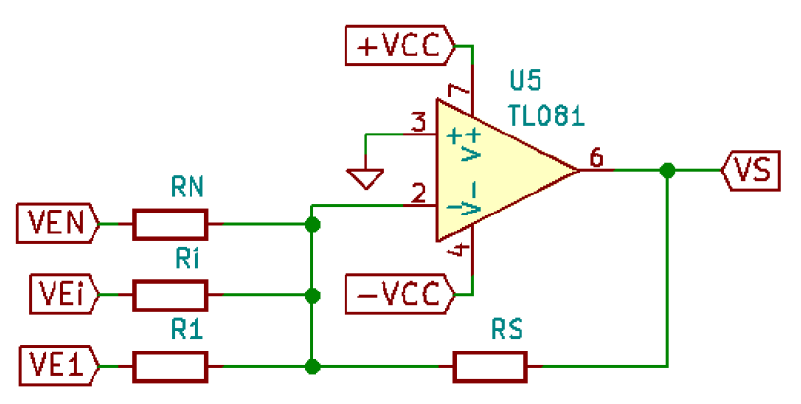
\includegraphics[width=10cm]{images/ali_ampli_somme.png}
\end{center}
}


%%%%%%%%%%%%%%%%%%%
\encadreTDExo{1.6 - Mettre en forme un capteur de température}{
On se propose d'étudier le circuit suivant :

\begin{center}
	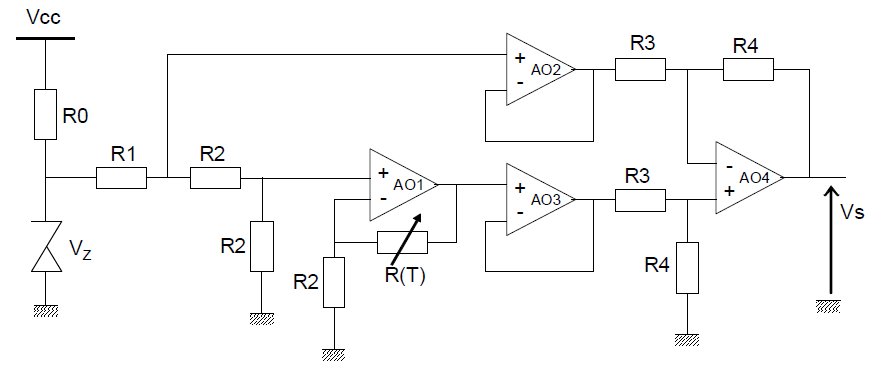
\includegraphics[width=16cm]{images/capteur_conditionnement.png}
\end{center}

La thermistance utilisée est de type PT100. La relation entre sa résistance (en Ohms) et la température (en \degre{}C) est la suivante :
$$R(T) = 100~(1 + 3.908×10^{-3} T - 5.802×10^{-7} T^2)$$

Une partie de la documentation de diodes Zener est fournie en annexe.
}

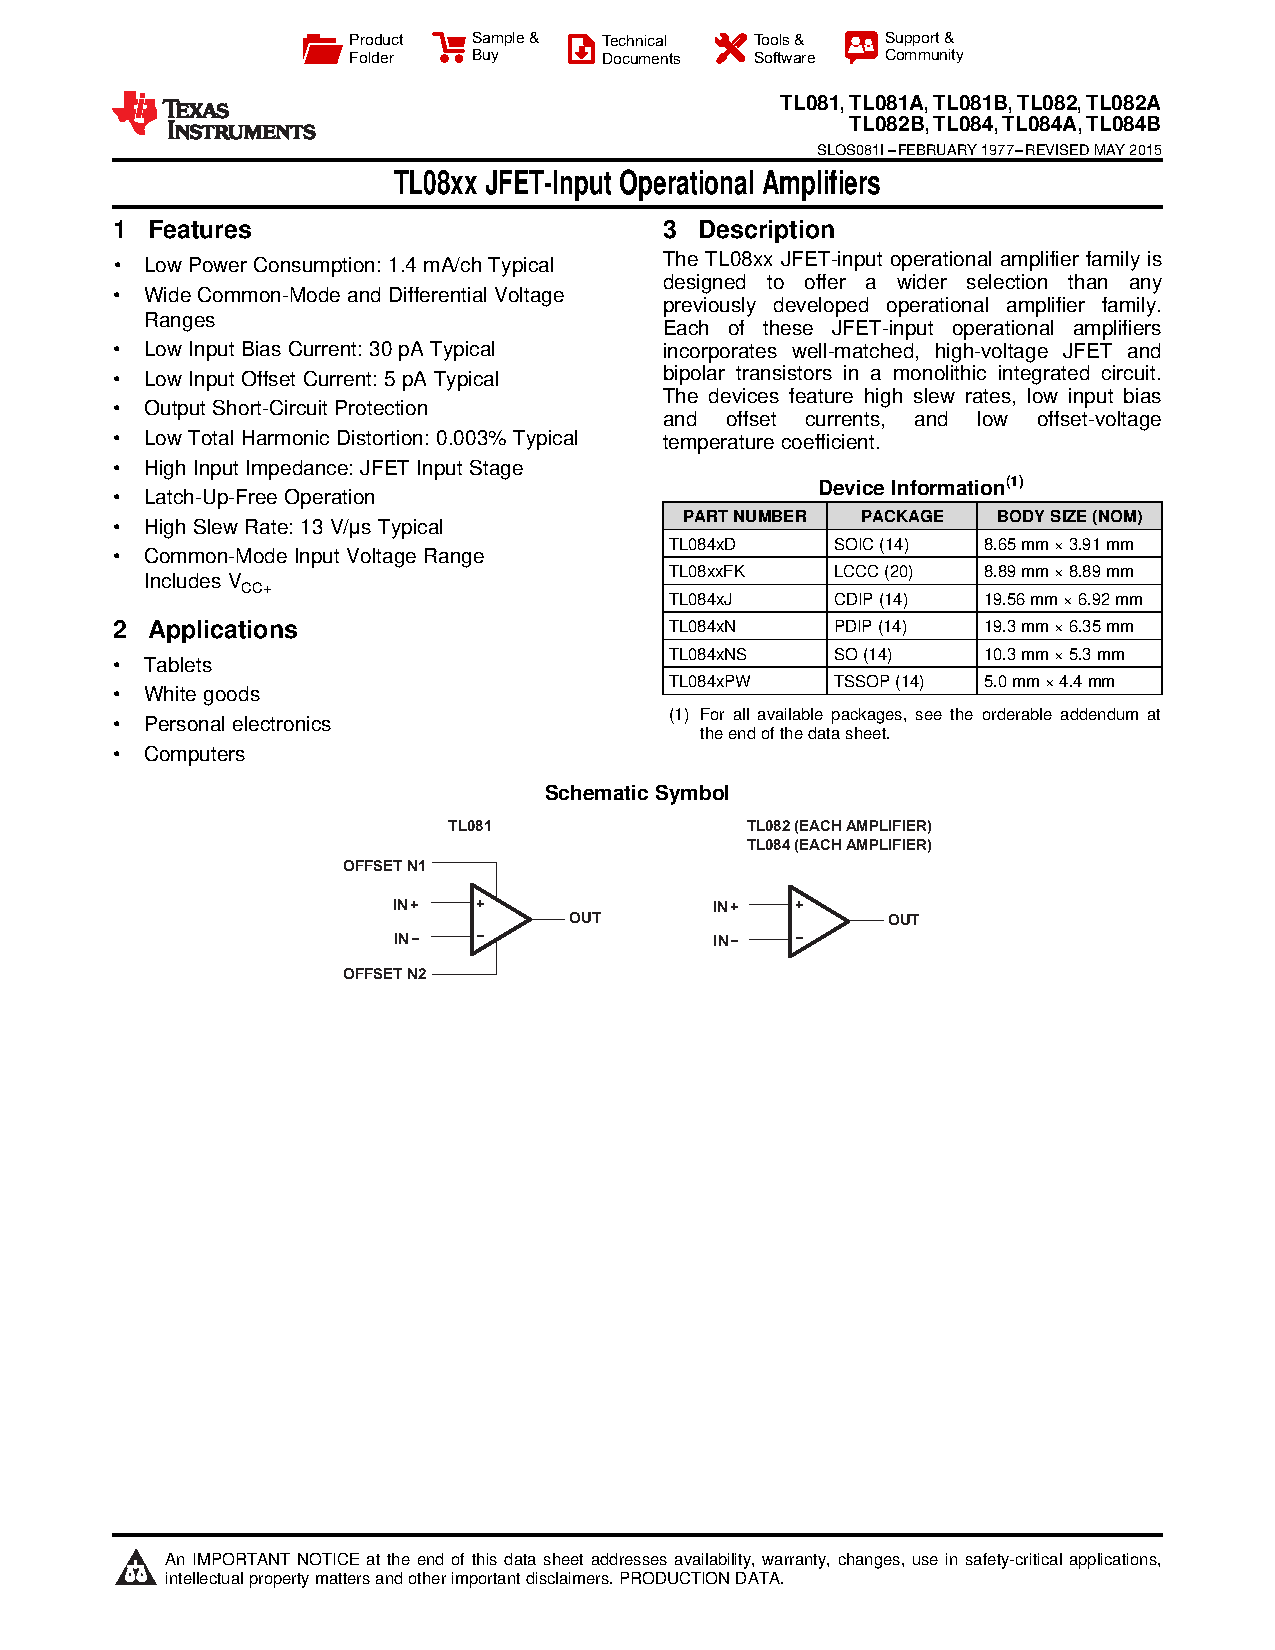
\includepdf[pages=-]{doc/doc_TL071_1p.pdf}
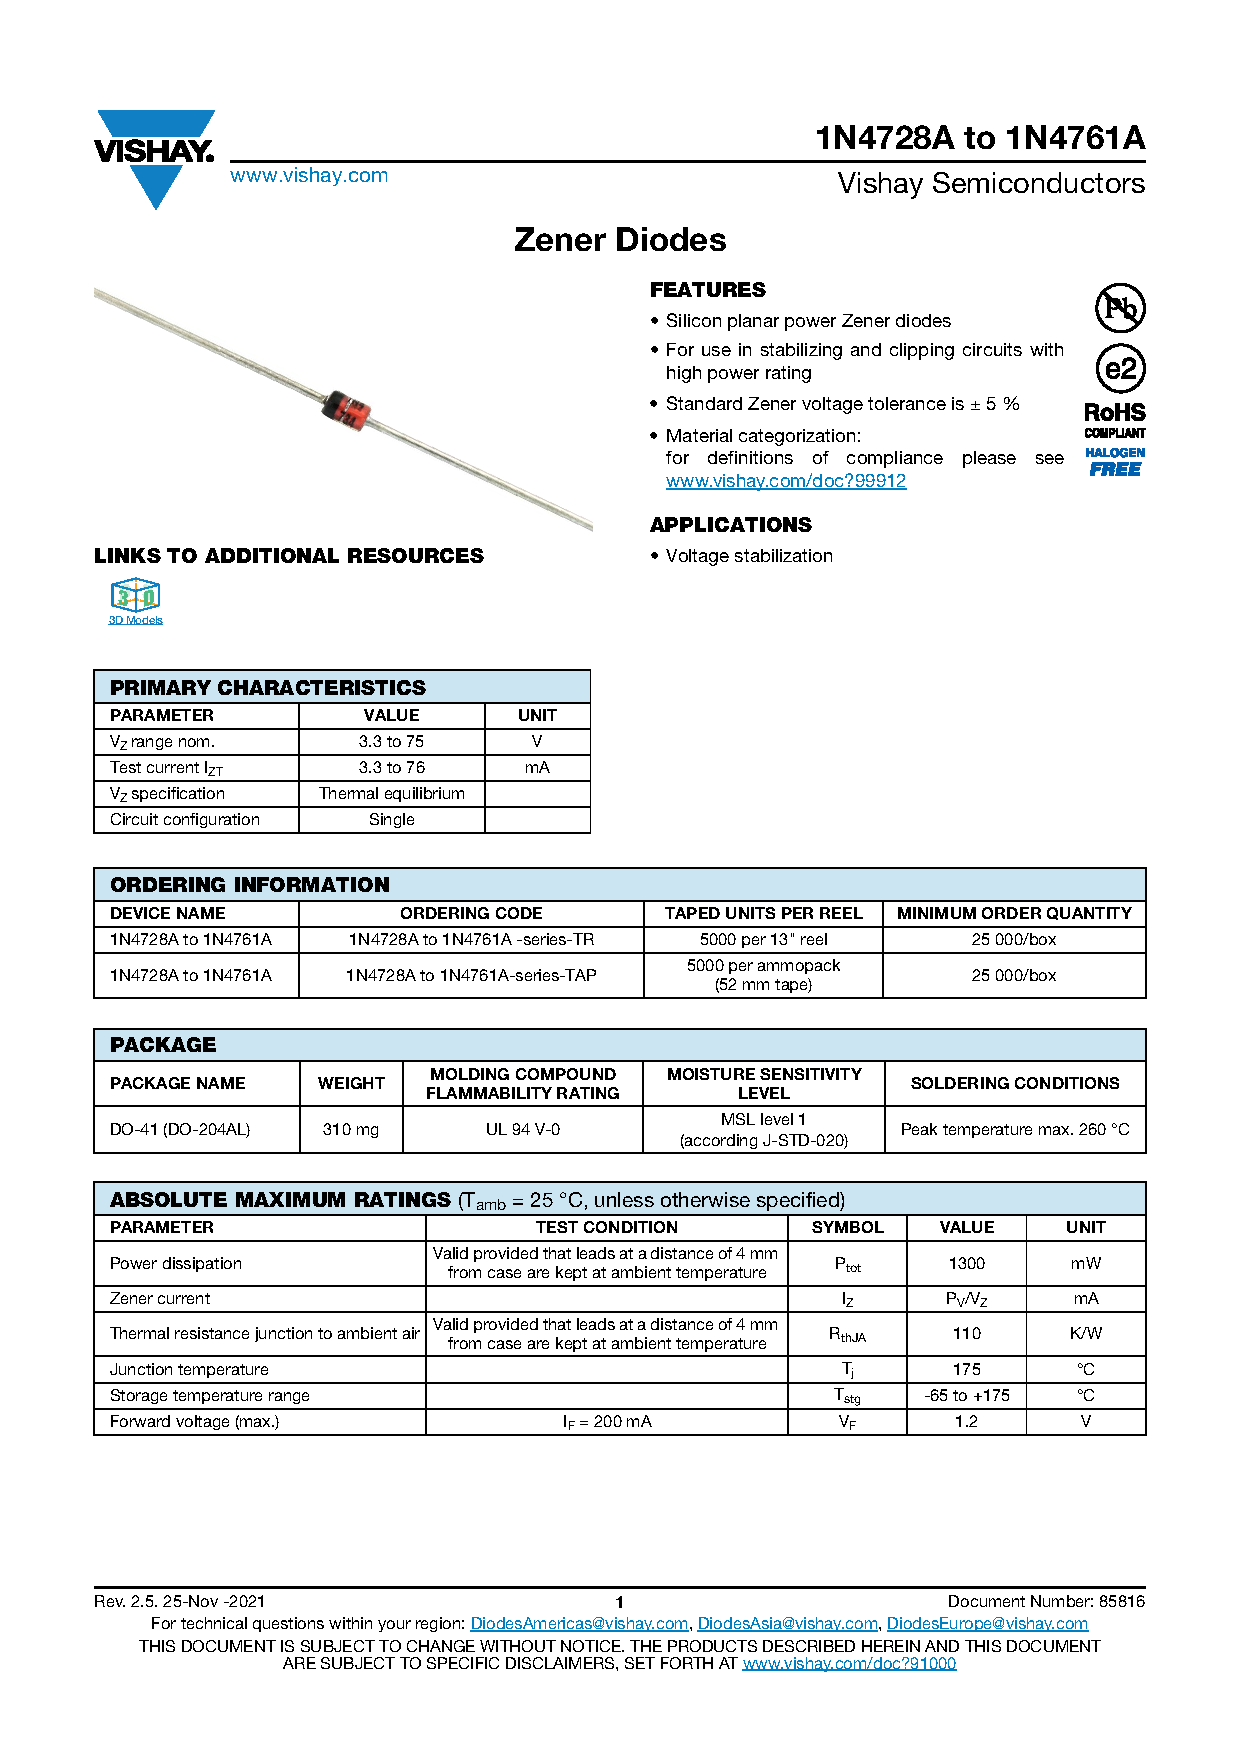
\includepdf[pages=1-2]{doc/1n4728a.pdf}

\end {document}